\section{Background of the Study}
	The urbanization of a settlement greatly changes its environment.
	In an urban city, the artificial surfaces, the physical structures, and man-made processes contribute to the modification of the city's climate.
	One effect of urbanization can be seen in the urban heat island, the phenomenon where urban areas have higher temperatures compared to nearby rural areas.
	Studies in over 400 cities worldwide have documented the urban heat island effect,
		with an average temperature of $\qtyrange{4}{5}{\degreeCelsius}$ more than their rural surroundings (\cite{Santamouris2020}).
	
	The urban heat island effect is attributed to the modifications that urbanization make to the energy balance of the area.
	Urban areas have different radiative, thermal, moisture, and aerodynamic properties compared to their rural surroundings.
	This is due to the shapes of buildings, the materials used in buildings, the removal of plants and soil, and air pollution (\cite{Stewart2012}).
	In addition to these urban modifications is anthropogenic heat, which is heat from man-made activities.
	Examples of anthropogenic heat include industrial processes, combustion of fuels in vehicles, and air-conditioning (\cite{Oke2017urban}).
	All of these contribute to the heating of the city.
	
	\begin{figure}
		\centering
		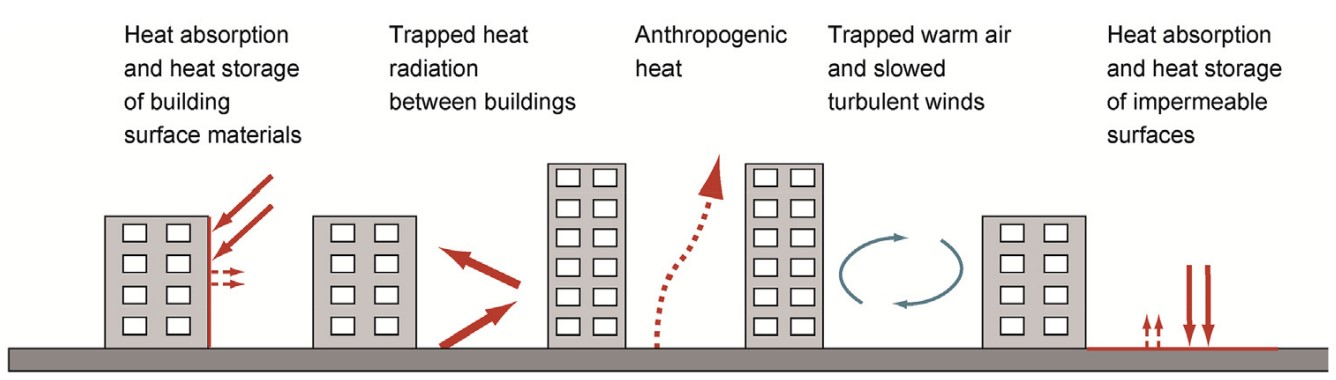
\includegraphics[width=\linewidth]{factors-of-urban-heat}
		\caption{
			Different factors that contribute to heat island formation in the tropical urban area.
			Taken from \textcite{Khan2021}, whom they have modified after \textcite{Kershaw2017}.
		}
		\label{fig:factors-of-urban-heat}
	\end{figure}
	
\section{Significance of the Study}
	One of these goals of the United Nations' Sustainable Development Goals (SDG) is SDG 11: Sustainable Cities and Communities.
	The goal is to ``make cities and human settlements inclusive, safe, resilient and sustainable'' (\cite{UN2015}).
	In line with SDG 11 is the mitigation of the urban heat island phenomenon, as it is a threat to the health of the citizens in the city.
	High temperatures can cause discomfort (\cite{Bhati2018}), worsen ambient air quality, and increase morbidity and mortality (\cite {Khan2021}).
	The effects of the urban heat island are also intensified by climate change.
	Thus, it is important to study this phenomenon in order to understand it better and to learn how to mitigate it.
	
	Cities are continually expanding, and new cities are being created as populations grow.
	We need cities that are resilient to disasters and extreme climate,
		especially with climate change intensifying these disasters.
	
	The urban heat island is also a threat to the health of the citizens in the city.
	This affects vulnerable sectors such as the young, the old, and those who are lower middle class and below.

\section{Objectives}
	The general objective of the study is to forecast the effect of the urban heat island in Metro Manila on air temperature.
	The specific objectives are:
	\begin{enumerate}
		\item to determine the performance of RegCM5 in simulating near-surface air temperature in Metro Manila;
		\item to analyze the trends of near-surface air temperature and urban heat island intensity in Metro Manila; and
		\item to forecast the near-surface air temperature and urban heat island intensity of Metro Manila to the year 2040.
		
	\end{enumerate}
	

\section{Scope and Delimitations}
	This study will focus on Metro Manila.
	This study will study two time periods: 
		the present represented by the years 2004 to 2023, 
		and the future represented by the years 2021 to 2040.
	
	The near-surface air temperature of Metro Manila will be analyzed.
	
	The RegCM software will be used for the simulations.
	RegCM is a free, limited area model for long-term regional climate simulation.
	The model is developed by the Abdus Salam International Centre for Theoretical Physics.
	The newest version, RegCM5, was released in 2023 and will be used in this study.
	This latest version is described in detail by \textcite{Giorgi2023}. 
	The previous version, RegCM4, was released in 2012 (\textcite{Giorgi2012}).
	
	The simulations will run on a few assumptions.
	The simulation will not model population increase.
	It will also assume that the urbanization of Metro Manila will remain fixed and that there will be no changes to the urban landscape throughout the simulation period.
	Anthropogenic heat will also be ignored in this study.